\documentclass{bschlangaul-aufgabe}
\bLadePakete{mathe,automaten,formale-sprachen,syntaxbaum}
\begin{document}
\bAufgabenMetadaten{
  Titel = {Reguläre Grammatik},
  Thematik = {Vorlesungsaufgaben},
  Referenz = THEO.Formale-Sprachen.Typ-3_Regulaer.Vorlesungsaufgaben-Regulaere-Grammatik,
  RelativerPfad = Module/70_THEO/10_Formale-Sprachen/10_Typ-3_Regulaer/Aufgabe_Vorlesungsaufgaben-Regulaere-Grammatik.tex,
  ZitatSchluessel = theo:fs:1,
  ZitatBeschreibung = {Seite 21},
  BearbeitungsStand = mit Lösung,
  Korrektheit = unbekannt,
  Ueberprueft = {unbekannt},
  Stichwoerter = {Reguläre Grammatik},
}

Gegeben ist eine Sprache $L \subset \Sigma^*$ mit \bAlphabet{a, b}. Zu
der Sprache $L$ gehören alle Wörter, die die Zeichenfolge $abba$
beinhalten.\index{Reguläre Grammatik}\footcite[Seite 21]{theo:fs:1}

\begin{enumerate}
\item Gib eine Grammatik an, die diese Sprache erzeugt.

% https://flaci.com/Gib2h94ar
\begin{bAntwort}
\bGrammatik{} mit \bAlphabet{a, b},
$S = S$,
$V = \{ S, A, B, C, D \}$

Tipp: Die Produktionsregeln so entwerfen, dass zuerst das Wort „abba“
erkannt wird, dann die Regeln entwerfen.

\begin{bProduktionsRegeln}
S -> aA | aS | bS,
A -> bB,
B -> bC,
C -> aD,
D -> aD | bD | epsilon
\end{bProduktionsRegeln}

Andere Möglichkeit:

\begin{bProduktionsRegeln}
S -> aA | aS | bS,
A -> bB,
B -> bC,
C -> aD | a,
D -> aD | bD | a | b
\end{bProduktionsRegeln}

Nicht erlaubt in regulärer Grammtik:

\begin{bProduktionsRegeln}
S -> abbaA
\end{bProduktionsRegeln}

\end{bAntwort}

\item Gib eine Ableitung/Syntaxbaum zu deiner Grammatik für das Wort
\texttt{aabbab} an.

\begin{bAntwort}
S $\rightarrow$
aS $\rightarrow$
aaA $\rightarrow$
aabB $\rightarrow$
aabbC $\rightarrow$
aabbaD $\rightarrow$
aabbabD $\rightarrow$
aabbab

\begin{center}
\begin{tikzpicture}[level distance=0.7cm]
\Tree [.S
  [.a ] [.S
    [.a ] [.A
      [.b ] [.B
        [.b ] [.C
          [.a ] [.D
            [.b ] [.D
              $\varepsilon$
              ]
            ]
          ]
        ]
      ]
    ]
  ]
]
\end{tikzpicture}
\end{center}
\end{bAntwort}
\end{enumerate}

\end{document}
